\chapter{Maxwells Equations}
\begin{enumerate}
	\item 	The $x$ and $z$-components of a static magnetic field in a region are $B_{x}=B_{0}\left(x^{2}-y^{2}\right)$ and $B_{z}=0$, respectively. Find one of the possible solution for its $y$-component which is consistent with the Maxwell equations?
	\item 	Which of the following expressions represent an electric field due to a time varying magnetic field?
	 \begin{tasks}(2)
		\task[\textbf{a.}]$K(x \hat{x}+\hat{y} \hat{y}+z \hat{z})$
		\task[\textbf{b.}]$K(x \hat{x}+y \hat{y}-z \hat{z})$
		\task[\textbf{c.}] $K(x \hat{x}-y \hat{y})$
		\task[\textbf{d.}] $K(y \hat{y}-x \hat{y}+2 z \hat{z})$
	\end{tasks}
	\item A uniform magnetic field in the positive $z$-direction passes through a circular wire loop of radius $1 \mathrm{~cm}$ and resistance $3.14 \Omega$ lying in the $x y$-plane. The field strength is reduced from 10 tesla to 9 tesla in $1 s$. Find the charge transferred across any point in the wire. 
	\item A small loop of wire of area $A=0.01 \mathrm{~m}^{2}, N=40$ turns and resistance $R=10 \Omega$ is initially kept in a uniform magnetic field $B$ in such a way that the field is normal to the loop. When it is pulled out of the magnetic field, a total charge of $Q=2 \times 10^{-5} C$ flows through the coil. Find the magnitude of the field $B$.
	\item A rectangular loop of dimension $L$ and width $w$ moves with a constant velocity $v$ away from an infinitely long straight wire carrying a current $I$ in the plane of the loop as shown in the figure below. Let $R$ be the resistance of the loop. Show that the current in the Toop at the instant the near side is at a distance $r$ from the wire is $\frac{\mu_{0} I L}{2 \pi R} \frac{w v}{r[r+w]}$.
	\begin{figure}[H]
		\centering
		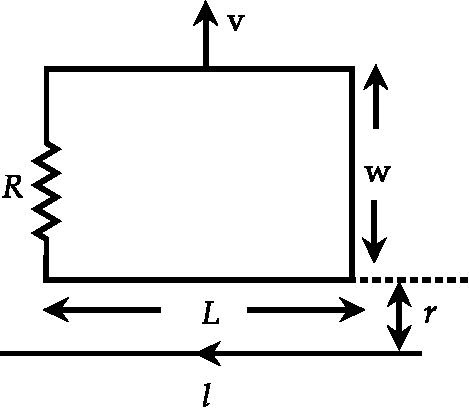
\includegraphics[height=3.5cm,width=4cm]{Ass-05}
	\end{figure}
\item A square loop of side $L$ and mass $M$ is made of a wire of cross-sectional area $A$ and resistance $R$ The loop. moving with a constant velocity $v_{v} \hat{i}$ in the horizontal xy-plane, enters a region $0 \leq x \leq 2 L$ having constant magnetic field $B \hat{k}$
\begin{figure}[H]
	\centering
	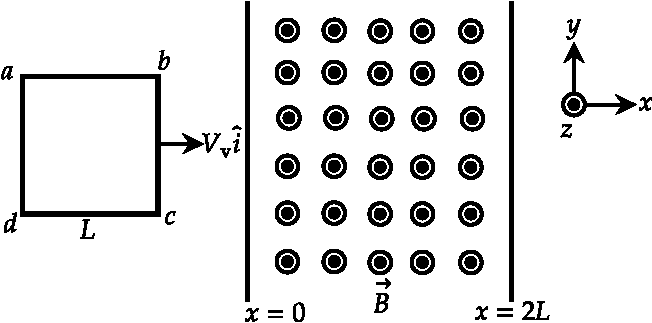
\includegraphics[height=4cm,width=8cm]{Ass-01}
\end{figure}
Find an expression for the $x$-component of the force $\vec{F}$ acting on the loop in terms of its velocity $\vec{v}(t), B, L$ and $R$.
\item A coil of 15 turns, each of radius 1 centimeter, is rotating at a constant angular velocity $\omega=300$ radians per second in a uniform magnetic field of $0.5$ tesla, as shown in the figure. Assume at time $t=0$ that the normal $\hat{n}$ to the coil plane is along the $y$-direction and that the self-inductance of the coil can be neglected. If the coil resistance is 9 ohms, what will be the magnitude of the induced current in milliamperes?
\begin{figure}[H]
	\centering
	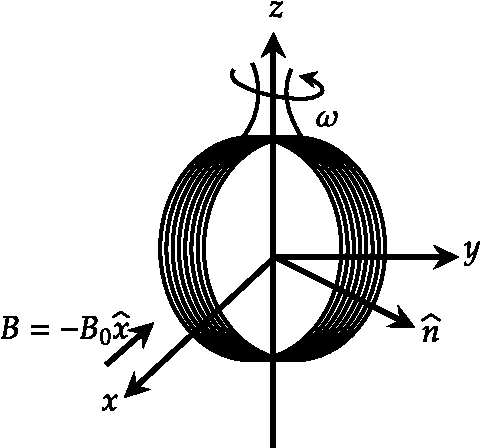
\includegraphics[height=3.8cm,width=4.3cm]{Ass-02}
\end{figure}
\item The circuit shown below is in a uniform magnetic lield that is into the page and is decreasing in magnitude at the rate of 150 Tesla/sec. Then tind the ammeter reading.
\begin{figure}[H]
	\centering
	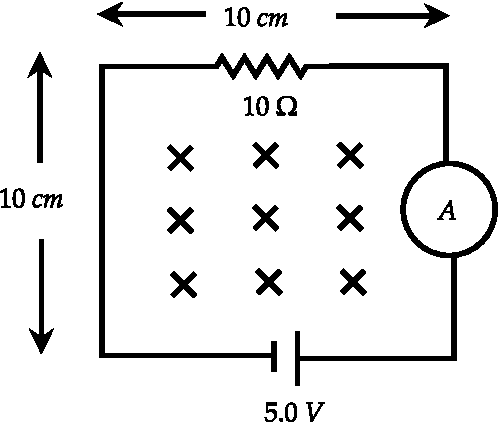
\includegraphics[height=4.5cm,width=5cm]{Ass-03}
\end{figure}
	\item A parallel plate air-gap capacitor is made up of two plates of area $10 \mathrm{~cm}^{2}$ each kept at a distance of $0.88 \mathrm{~mm}$. A sine wave of amplitude $10 \mathrm{~V}$ and frequency $50 \mathrm{~Hz}$ is applied across the capacitor as shown in the figure.
	 \begin{tasks}(1)
		\task[\textbf{a.}]Find the amplitude of the displacement current density between the plates.
		\task[\textbf{b.}]
		(b) Find the r.m.s value of the displacement current density between the plates.
		\task[\textbf{c.}]Find the average value of the displacement current density (in $\mathrm{mA} / \mathrm{m}^{2}$ ) between the plates.
	\end{tasks}
\begin{figure}[H]
	\centering
	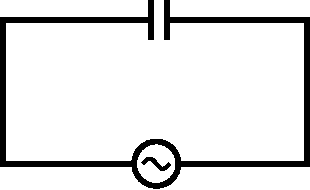
\includegraphics[height=2.5cm,width=4cm]{Ass-04}
\end{figure}
	\item Consider a capacitor placed in free space, consisting of two concentric circular parallel plates of radii $r$. The separation $z$ between the plates oscillates with a constant frequency $\omega$, i.e. $z(t)=z_{0}+z_{1} \cos \omega t$. Here $z_{0}$ and $z_{1}\left(<z_{0}\right)$ are constants. The separation $z(t)$ $(<<r)$ is varied in such a way that the voltage $V_{0}$ across the capacitor remains constant,\\
	(a) Calculate the displacement current density and the displacement current between the plates through a concentric circle of radius $r / 2$.\\
	(b) Calculate the magnetic field vector $(\vec{H})$ between the plates at-a distance $r / 2$ from the axis of the capacitor.

	
	
	
	
	
	
	
	
	
	
	
\end{enumerate}